\documentclass[aspectratio=32]{beamer}

\usepackage{beamerthemesplit}
\usetheme{Boadilla}
\usecolortheme{dolphin}
\usefonttheme{serif}

\usepackage{multirow}
\usepackage{subfig}
\usepackage{amssymb,amsmath,mathtools}
\usepackage{amsfonts,booktabs}
\usepackage{lmodern,textcomp}
\usepackage{color}
\usepackage{tikz}
\usetikzlibrary{arrows.meta,calc,positioning,shapes.geometric}
\usepackage{multicol}
\usepackage{graphicx}
\usepackage{ctex}
\usepackage{hyperref}
\usepackage{nicefrac}
\usepackage{tabularx}
\usepackage{ragged2e}

\graphicspath{{material/}}
\setbeamertemplate{navigation symbols}{}
\setbeamertemplate{caption}[numbered]
\setbeamercolor{structure}{fg=blue!70!black}
\setbeamercolor{frametitle}{fg=blue!70!black}
\setbeamerfont{frametitle}{size=\large}
\setlength{\parskip}{2pt}
\setlength{\tabcolsep}{5pt}

\definecolor{LectureBlue}{RGB}{18,18,150}
\definecolor{SoftBlue}{RGB}{235,240,255}
\definecolor{SoftRed}{RGB}{255,239,239}
\definecolor{SoftGreen}{RGB}{235,249,240}
\setbeamercolor{lecturesection}{fg=white,bg=LectureBlue}
\newcommand{\lecturesectionpage}[1]{%
\begin{frame}[plain]
\begin{center}
\vfill
\begin{beamercolorbox}[wd=0.74\textwidth,rounded=true,shadow=true,center,sep=1em]{lecturesection}
\LARGE #1
\end{beamercolorbox}
\vfill
\end{center}
\end{frame}
}

\title[Lecture 5: Quality Ladder]{Lecture 5：质量阶梯与创造性破坏}
\author{陈宠\inst{1}}
\institute{中国人民大学经济学院\inst{1}}
\date{2026 年秋季}

\begin{document}

% 1
\begin{frame}
\maketitle
\end{frame}

% 2
\begin{frame}{目录}
\tableofcontents[hideallsubsections]
\vspace{0.25cm}
\begin{center}
\textcolor{LectureBlue}{从品种扩张到质量升级：创新如何替代现任者并推动增长}
\end{center}
\end{frame}

\section{从品种扩张到质量阶梯}
\lecturesectionpage{从品种扩张到质量阶梯}

% 3
\begin{frame}{两种内生增长机制}
\small
\begin{columns}[T]
\column{0.47\textwidth}
\begin{block}{Romer：品种扩张}
\[
  Y=H_Y^{1-\alpha}\int_0^A x(i)^\alpha di
\]
研发创造新的产品品种，$A$ 增加；已有品种通常继续存在。
\end{block}
\column{0.47\textwidth}
\begin{block}{质量阶梯}
\[
  q_j=\lambda_q^j q_0,\qquad \lambda_q>1
\]
创新提高同一产品线的质量，新的领先者替代旧的垄断者。
\end{block}
\end{columns}
\vspace{0.18cm}
\begin{alertblock}{本讲的选择}
正式推导 Aghion--Howitt 的单一质量阶梯；Grossman--Helpman 仅作为多产品线文献定位，不混用两套均衡公式。
\end{alertblock}
\end{frame}

% 4
\begin{frame}{质量升级的经济事实}
\small
\begin{itemize}
  \item 企业进入与退出并存：新企业成功后获得短期租金，旧企业被替代。
  \item 产品质量不是一次性提高，而是沿着阶梯反复升级。
  \item 研发成功具有不确定性；失败并不改变当前产品线的状态。
  \item 专利竞赛把“提高质量”转成“夺取下一期垄断位置”的动态竞争。
\end{itemize}
\vspace{0.18cm}
\begin{center}
\begin{tikzpicture}[>=Latex,scale=0.82]
\foreach \x/\lab in {0/$q_j$,2/$q_{j+1}$,4/$q_{j+2}$,6/$q_{j+3}$}
  {\node[draw,rounded corners,fill=SoftBlue,minimum width=1.25cm,minimum height=0.62cm] (n\x) at (\x,0) {\lab};}
\draw[->,very thick,LectureBlue] (n0)--node[above]{$\lambda_q$}(n2);
\draw[->,very thick,LectureBlue] (n2)--node[above]{$\lambda_q$}(n4);
\draw[->,very thick,LectureBlue] (n4)--node[above]{$\lambda_q$}(n6);
\end{tikzpicture}
\end{center}
\end{frame}

% 5
\begin{frame}{文献地图：从 Schumpeter 到 Aghion--Howitt}
\small
\begin{enumerate}
  \item \textbf{Schumpeter：}创新与企业家进入改变市场结构，增长伴随创造性破坏。
  \item \textbf{专利竞赛：}研发成功概率决定谁获得下一期垄断权。
  \item \textbf{Grossman--Helpman：}把质量升级放在多个产品线上，强调创新与贸易联系。
  \item \textbf{Aghion--Howitt（1992）：}用 Poisson 创新到达与现任者价值函数，把垄断租金、研发和增长闭合。
\end{enumerate}
\begin{block}{分析重点}
质量阶梯的关键不是“$q$ 更高”这一静态事实，而是创新成功会让未来垄断者获得租金、并让当前租金终止。
\end{block}
\end{frame}

% 6
\begin{frame}{Grossman--Helpman 的位置：多产品线升级}
\small
\begin{columns}[T]
\column{0.48\textwidth}
\begin{block}{多产品线}
经济中存在许多产品线，每一条产品线都有自己的质量状态和创新竞赛。
\end{block}
\column{0.48\textwidth}
\begin{block}{与本讲的区别}
本讲只使用 Aghion--Howitt 的单一代表性质量阶梯，不把多产品线的聚合条件写入其均衡。
\end{block}
\end{columns}
\vspace{0.2cm}
\begin{alertblock}{为什么单独定位？}
文献中的相似术语不意味着模型相同。先明确产品线结构，再决定状态变量、创新率和福利函数如何定义。
\end{alertblock}
\end{frame}

% 7
\begin{frame}{Poisson 过程：为什么适合描述创新到达？}
\small
令研发努力为 $z$，创新到达率为
\[
  \boxed{\tau(z)=\mu z},\qquad \mu>0.
\]
短时间 $dt$ 内：
\[
  \Pr(\text{创新})=\mu z\,dt+o(dt),
  \qquad
  \Pr(\text{不创新})=1-\mu z\,dt+o(dt).
\]
\begin{itemize}
  \item 无记忆性：过去失败不会改变下一瞬间的到达概率。
  \item 等待时间 $T$ 服从指数分布，$\mathbb{E}T=1/(\mu z)$。
  \item 可解性代价：线性到达率忽略了研发团队内部的复杂互动和拥堵。
\end{itemize}
\end{frame}

\section{Aghion--Howitt：创造性破坏}
\lecturesectionpage{Aghion--Howitt：创造性破坏}

% 8
\begin{frame}{论文与核心机制}
\small
\begin{columns}[T]
\column{0.56\textwidth}
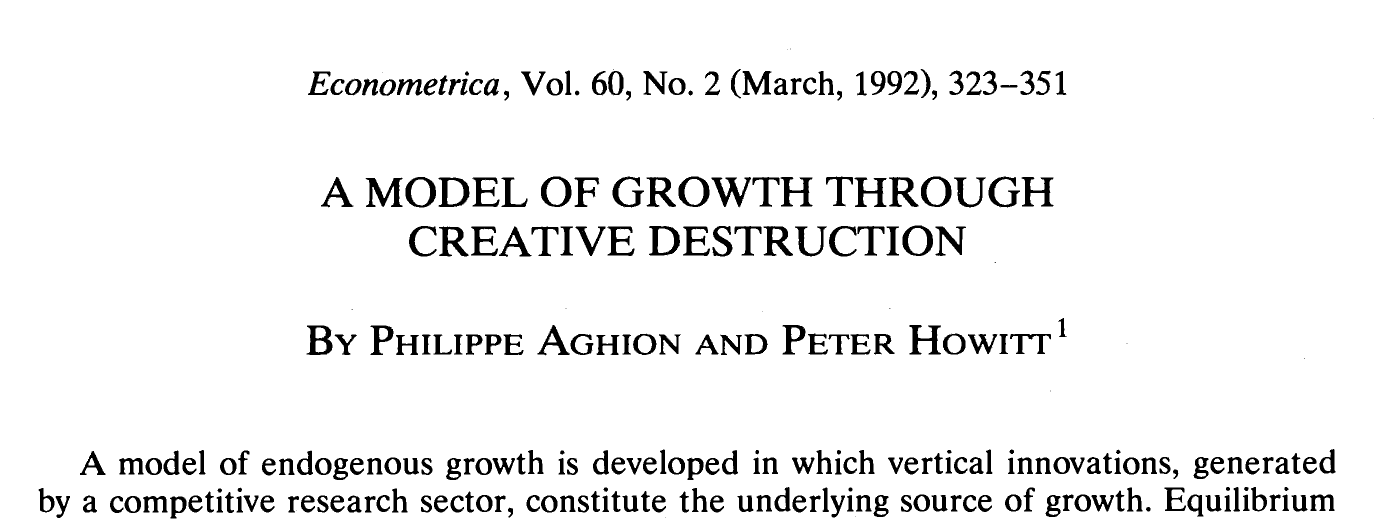
\includegraphics[width=\linewidth]{aghion_howitt1992_title}
\column{0.40\textwidth}
\begin{block}{核心问题}
创新者为什么愿意投入研发？创新如何转化为长期增长？
\end{block}
\begin{itemize}
  \item 成功创新将质量提高为 $\lambda_q q_j$。
  \item 新创新者获得垄断利润，旧创新者被创造性破坏。
\end{itemize}
\end{columns}
\vspace{0.06cm}
\scriptsize\textcolor{gray}{来源：Aghion and Howitt（1992）标题页；原 PDF 第 2 页，期刊第 323 页。}
\end{frame}

% 9
\begin{frame}{产品线、企业与劳动}
\small
每个时期只有一个领先质量 $q_j$ 的中间品企业：
\[
  q_j=\lambda_q^j q_0,qquad \lambda_q>1.
\]
生产劳动 $x_j$ 生产中间品，研发劳动 $z_j$ 参加创新竞赛：
\[
  \boxed{x_j+z_j=L}.
\]
\begin{itemize}
  \item 现任垄断者选择 $x_j$，获得当前利润 $\pi_j$。
  \item 潜在进入者选择 $z_j$，以概率 $\mu z_jdt$ 在 $dt$ 内取得下一阶创新。
  \item $L$ 固定是为了把重点放在质量增长与创造性破坏，而不是人口扩张。
\end{itemize}
\end{frame}

% 10
\begin{frame}{课堂记号与原文记号的对应}
\scriptsize
\begin{table}
\centering
\begin{tabular}{p{0.27\textwidth}p{0.28\textwidth}p{0.33\textwidth}}
\toprule
课堂记号 & 原文常用记号 & 经济含义 \\
\midrule
$q_j=\lambda_q^j q_0$ & $A_j=\gamma^jA_0$ & 第 $j$ 阶质量水平 \\
$\lambda_q>1$ & $\gamma>1$ & 一次成功创新的质量步长 \\
$\tau(z)=\mu z$ & $\lambda\phi(n,R)$ & 创新到达率；课堂采用线性研究技术 \\
$z$ & $n$ 或 $R$ & 研发劳动投入 \\
$x$ & $x$ & 中间品生产投入 \\
\bottomrule
\end{tabular}
\end{table}
\vspace{0.15cm}
\begin{alertblock}{记号纪律}
以下推导统一使用 $q_j,\lambda_q,\mu,z$；原文符号只在本页用于定位，避免把多产品线模型的 $A_j$ 与 Romer 的蓝图数量混为一谈。
\end{alertblock}
\end{frame}

% 11
\begin{frame}{生产端：质量乘上中间品数量}
\small
最终消费品由中间品服务生产：
\[
  \boxed{Y_j=q_jF(x_j)},\qquad F'>0,\quad F''<0.
\]
劳动约束：
\[
  x_j+z_j=L.
\]
\begin{itemize}
  \item $q_j$ 提高会使同样的 $x_j$ 产生更多最终品。
  \item $F$ 的凹性使垄断者面对向下倾斜的需求，并产生有限的最优生产量。
  \item 研发劳动 $z_j$ 不直接出现在当前产出中，而是提高下一次创新的到达率。
\end{itemize}
\begin{block}{一个清晰的机会成本}
增加一个单位 $z$ 会减少一个单位 $x$，降低当前利润；它的收益是提高未来夺取垄断租金的概率。
\end{block}
\end{frame}

% 12
\begin{frame}{中间品市场：反需求与垄断者问题}
\small
最终品价格归一化为 $1$，则中间品的反需求为其边际产品：
\[
  \boxed{p_j=q_jF'(x_j)}.
\]
若中间品生产的单位工资为 $w_j$，垄断者选择 $x_j$ 最大化
\[
  \pi_j=\max_{x\geq0}\,[q_jF'(x)-w_j]x.
\]
一阶条件为
\[
  q_j\big[F'(x_j)+x_jF''(x_j)\big]=w_j.
\]
\begin{alertblock}{经济含义}
垄断者把边际收益产品与边际成本比较，但还要考虑增加产量会压低全部已售中间品的价格。
\end{alertblock}
\end{frame}

% 13
\begin{frame}{Cobb--Douglas 特例：价格和利润}
\small
令 $F(x)=x^\alpha$，$0<\alpha<1$：
\[
  p_j=q_j\alpha x_j^{\alpha-1}.
\]
一阶条件给出固定加成：
\[
  \boxed{p_j=\frac{w_j}{\alpha}}.
\]
由此得到生产量与利润：
\begin{align*}
  x_j&=\left(\frac{\alpha^2q_j}{w_j}\right)^{\frac{1}{1-\alpha}},\\
  \pi_j&=(p_j-w_j)x_j
  =\frac{1-\alpha}{\alpha}w_jx_j.
\end{align*}
\begin{block}{质量的作用}
$q_j$ 越高，给定工资下的需求与利润越高；但利润只持续到下一次创新到达。
\end{block}
\end{frame}

% 14
\begin{frame}{质量状态的跳跃：创新替代现任者}
\small
\begin{center}
\begin{tikzpicture}[>=Latex,scale=0.84]
\node[draw,rounded corners,fill=SoftBlue,minimum width=1.8cm,minimum height=0.65cm] (q0) at (0,0) {$q_j$};
\node[draw,rounded corners,fill=SoftGreen,minimum width=1.8cm,minimum height=0.65cm] (q1) at (3.2,0) {$q_{j+1}=\lambda_qq_j$};
\node[draw,rounded corners,fill=SoftRed,minimum width=1.8cm,minimum height=0.65cm] (q2) at (6.4,0) {$q_{j+2}$};
\draw[->,very thick] (q0)--node[above]{成功创新}(q1);
\draw[->,very thick] (q1)--node[above]{成功创新}(q2);
\node at (1.6,-0.8) {现任者垄断租金};
\node at (4.8,-0.8) {新进入者接管};
\end{tikzpicture}
\end{center}
\vspace{0.16cm}
\begin{itemize}
  \item 创新发生前，现任者享有 $q_j$ 对应的利润流。
  \item 创新发生瞬间，质量跃升，新的创新者获得下一阶专利。
  \item 因而当前垄断租金的终止风险正是研发的私人收益来源。
\end{itemize}
\end{frame}

% 15
\begin{frame}{Poisson 到达与等待时间}
\small
给定恒定研发努力 $z$，创新事件过程为
\[
  N_t\sim\operatorname{Poisson}(\mu zt).
\]
第一次创新等待时间 $T$ 的生存函数为
\[
  \Pr(T>t)=e^{-\mu zt},
  \qquad \mathbb{E}T=\frac{1}{\mu z}.
\]
\begin{columns}[T]
\column{0.47\textwidth}
\begin{block}{提高 $z$}
创新更快到达，平均等待时间更短；但研发劳动从当前生产中抽离。
\end{block}
\column{0.47\textwidth}
\begin{block}{提高 $\mu$}
同样的研发投入更有效；它可以代表科研基础设施、知识工具或制度效率。
\end{block}
\end{columns}
\end{frame}

% 16
\begin{frame}{创新事件的时间线}
\small
\begin{center}
\begin{tikzpicture}[>=Latex,scale=0.76]
\draw[very thick,->] (0,0)--(9,0) node[right]{时间};
\draw[fill=SoftBlue] (1.2,-0.2) rectangle (2.8,0.2);
\draw[fill=SoftGreen] (4.0,-0.2) rectangle (5.6,0.2);
\draw[fill=SoftRed] (7.0,-0.2) rectangle (8.3,0.2);
\node at (2.0,0.65) {$q_j$ 垄断};
\node at (4.8,0.65) {$q_{j+1}$ 垄断};
\node at (7.65,0.65) {$q_{j+2}$ 垄断};
\draw[->,thick] (2.8,0)--(4.0,0);
\draw[->,thick] (5.6,0)--(7.0,0);
\node[above] at (3.4,0.05) {创新};
\node[above] at (6.3,0.05) {创新};
\end{tikzpicture}
\end{center}
\vspace{0.22cm}
\begin{block}{动态对象}
现任者的价值等于“在下一次创新到达前获得的利润流”；下一次创新的价值又取决于新的质量和工资。
\end{block}
\end{frame}

% 17
\begin{frame}{现任者的价值：创造性破坏进入分母}
\small
若下一次创新的到达率为 $\mu z_{j+1}$，现任者每期利润为 $\pi_{j+1}$，则
\[
  V_{j+1}=\int_0^\infty e^{-rt}e^{-\mu z_{j+1}t}\pi_{j+1}\,dt.
\]
积分得到
\[
  \boxed{V_{j+1}=\frac{\pi_{j+1}}{r+\mu z_{j+1}}}.
\]
\begin{itemize}
  \item $r$ 是时间贴现：越不看重未来，资产价值越低。
  \item $\mu z_{j+1}$ 是创造性破坏率：越可能快速被替代，当前专利寿命越短。
  \item 这与无风险永续资产 $\pi/r$ 不同，分母多出创新终止风险。
\end{itemize}
\end{frame}

% 18
\iffalse
\begin{frame}{HJB 直觉：价值增长与价值毁灭}
\small
把价值写成连续时间 HJB：
\[
  rV_{j+1}=\pi_{j+1}-\mu z_{j+1}V_{j+1}
  +\mu z_{j+1}V_{j+2}.
\]
在“现任者被下一代创新替代”的竞争中，现任者只保留到达下一次创新前的租金；将价值的状态跳跃整理后，得到上一页的资产定价：
\[
  (r+\mu z_{j+1})V_{j+1}=\pi_{j+1}.
\]
\begin{alertblock}{关键机制}
未来研发越强，当前垄断租金越容易被终止，当前专利价值越低；这会反过来影响今天的研发激励。
\end{alertblock}
\end{frame}
\fi

% 19
\begin{frame}{研发自由进入：工资等于成功概率乘价值}
\small
一名研发者增加 $dz$，使短时间创新概率增加 $\mu dz\,dt$。其边际收益为 $\mu V_{j+1}$，边际成本是研发工资 $w_R$：
\[
  \boxed{w_R=\mu V_{j+1}}\qquad\text{（正研发的自由进入条件）}.
\]
若 $w_R>\mu V_{j+1}$，研发退出；若 $w_R<\mu V_{j+1}$，更多进入者会把工资推高或把可用劳动推低。
\begin{block}{与 Romer 的对照}
Romer 中研发创造新蓝图，收益来自新产品租金；Aghion--Howitt 中研发提高夺取下一阶垄断的概率，收益还要扣除创造性破坏导致的租金寿命缩短。
\end{block}
\end{frame}

% 20
\begin{frame}{劳动市场闭合：当前研发依赖未来价值}
\small
劳动市场为
\[
  x_j+z_j=L.
\]
生产端给出 $x_j$ 与 $w_j$ 的关系；研发自由进入给出 $w_R=\mu V_{j+1}$；价值函数给出
\[
  V_{j+1}=\frac{\pi_{j+1}}{r+\mu z_{j+1}}.
\]
因此当前研发满足一条向前看的关系：
\[
  w_R=\mu\frac{\pi_{j+1}}{r+\mu z_{j+1}}.
\]
\begin{alertblock}{为什么是“向前看”？}
今天投入研发的回报是明天质量阶梯上的垄断利润；而明天的研发又决定明天之后多久发生再次替代。
\end{alertblock}
\end{frame}

% 21
\begin{frame}{Aghion--Howitt Figure 1：未来研发压低当前价值}
\small
\begin{columns}[T]
\column{0.58\textwidth}
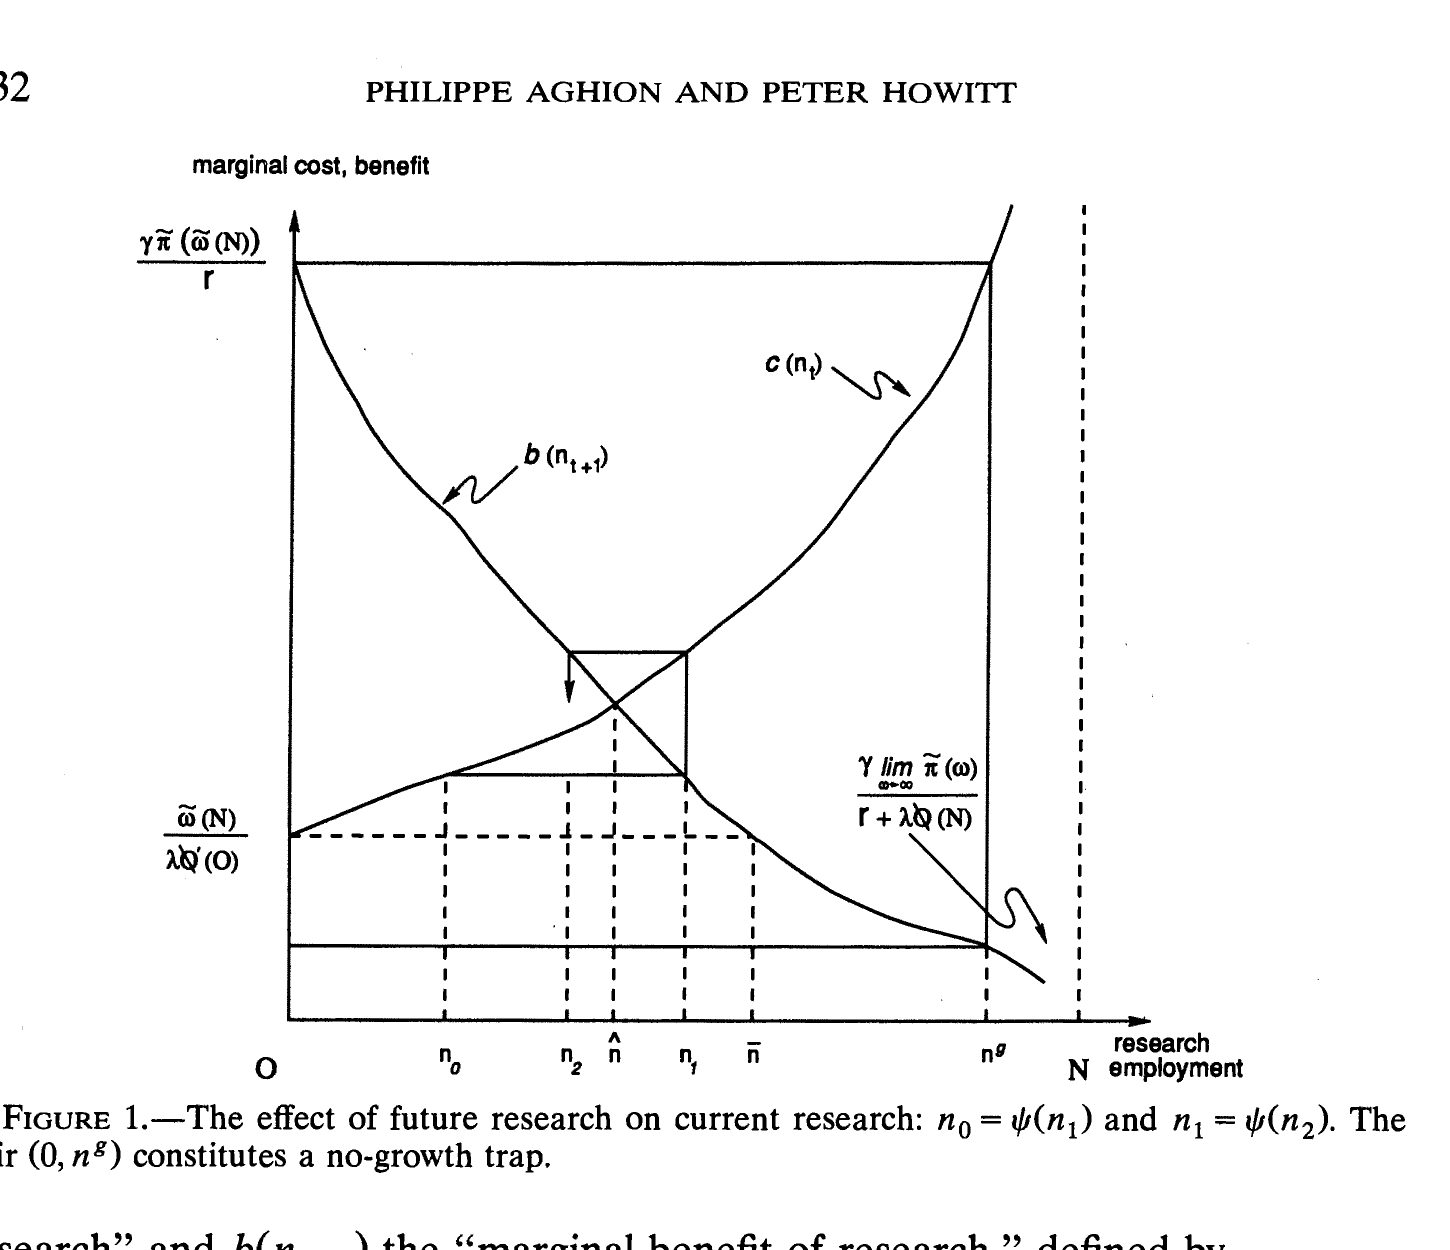
\includegraphics[width=\linewidth]{aghion_howitt1992_fig1_research_dynamics}
\column{0.38\textwidth}
\begin{itemize}
  \item 横轴是研发就业，纵轴是边际成本或边际收益。
  \item $c(n_{t+1})$ 表示未来研发的影响，改变当前研发的收益。
  \item 当未来创新越快，当前专利越容易被替代，当前研发激励会发生变化。
\end{itemize}
\begin{block}{图中风险}
低研发可能对应无增长陷阱；均衡是否存在、是否唯一，取决于价值与成本曲线的交点。
\end{block}
\end{columns}
\vspace{0.02cm}
\scriptsize\textcolor{gray}{来源：Aghion and Howitt（1992），Figure 1；原 PDF 第 11 页，期刊第 332 页。}
\end{frame}

% 22
\begin{frame}{平衡增长与无增长陷阱}
\small
\begin{itemize}
  \item 在平衡增长路径上，劳动分配 $z$ 稳定，创新到达率 $\mu z$ 稳定。
  \item 若质量每次乘以 $\lambda_q$，创新事件是离散跳跃，长期增长率来自事件频率和步长的组合。
  \item 如果研发回报始终低于机会成本，$z=0$ 是角点；创新停止，质量和产出不再增长。
\end{itemize}
\begin{center}
\begin{tikzpicture}[>=Latex,scale=0.78]
\node[draw,rounded corners,fill=SoftRed,minimum width=2.4cm,minimum height=0.7cm] (z0) at (0,0) {$z=0$};
\node[draw,rounded corners,fill=SoftBlue,minimum width=2.8cm,minimum height=0.7cm] (z) at (4,0) {$0<z<L$};
\node[draw,rounded corners,fill=SoftGreen,minimum width=2.4cm,minimum height=0.7cm] (g) at (8,0) {持续增长};
\draw[->,thick] (z0)--node[above]{克服进入成本}(z);
\draw[->,thick] (z)--node[above]{创新到达}(g);
\end{tikzpicture}
\end{center}
\end{frame}

% 23
\begin{frame}{对数质量的增长率}
\small
经过 $N_t$ 次创新后，质量为
\[
  q_t=q_0\lambda_q^{N_t}.
\]
取对数：
\[
  \ln q_t=\ln q_0+N_t\ln\lambda_q.
\]
由于 $\mathbb{E}N_t=\mu zt$，所以期望对数质量的增长率是
\[
  \boxed{g_{\ln q}=\frac{d\,\mathbb{E}[\ln q_t]}{dt}
  =\mu z\ln\lambda_q}.
\]
\begin{block}{分解}
增长 = 创新到达频率 $\mu z$ $\times$ 每次创新的对数步长 $\ln\lambda_q$。
\end{block}
\end{frame}

% 24
\begin{frame}{质量水平的增长率：Poisson 矩母函数}
\footnotesize
Poisson 变量的矩母函数给出
\[
  \mathbb{E}[\lambda_q^{N_t}]
  =\exp\left[\mu zt(\lambda_q-1)\right].
\]
因此
\[
  \mathbb{E}[q_t]
  =q_0\exp\left[\mu zt(\lambda_q-1)\right],
\]
从而
\[
  \boxed{g_{\mathbb{E}q}=\mu z(\lambda_q-1)}.
\]
\begin{alertblock}{两种增长率的差别}
\[
  \ln\lambda_q<\lambda_q-1\quad(\lambda_q>1).
\]
当创新步长很小时，$\ln\lambda_q\approx\lambda_q-1$；步长较大时，不能把两者混用。
\end{alertblock}
\end{frame}

\section{福利与政策}
\lecturesectionpage{福利与政策：创新激励与垄断扭曲}

% 25
\begin{frame}{教学化社会规划者问题}
\small
令当前研发劳动为 $z$，生产劳动为 $L-z$，采用质量增长的水平口径。规划者最大化消费的现值：
\[
  \boxed{U(z)=\frac{q_0F(L-z)}{r-\mu z(\lambda_q-1)}}.
\]
这里要求
\[
  r>\mu z(\lambda_q-1),
\]
以保证增长调整后的现值有限。
\begin{itemize}
  \item 分子：减少生产劳动会降低当前消费。
  \item 分母：研发提高未来质量增长，降低有效贴现负担。
  \item 这是教学化目标，用来展示增长收益与当前产出损失的权衡，不替代完整一般均衡福利函数。
\end{itemize}
\end{frame}

% 26
\begin{frame}{规划者的一阶条件}
\small
对 $U(z)$ 取对数：
\[
  \ln U(z)=\ln q_0+\ln F(L-z)-\ln\big[r-\mu z(\lambda_q-1)\big].
\]
对 $z$ 求导并令其为零：
\[
  -\frac{F'(L-z)}{F(L-z)}
  +\frac{\mu(\lambda_q-1)}{r-\mu z(\lambda_q-1)}=0.
\]
因此内点条件为
\[
  \boxed{\frac{F'(L-z)}{F(L-z)}
  =\frac{\mu(\lambda_q-1)}{r-\mu z(\lambda_q-1)}}.
\]
\begin{block}{左边与右边}
左边是从生产中抽出一个劳动者的产出损失；右边是研发提高质量增长所带来的现值收益。
\end{block}
\end{frame}

% 27
\begin{frame}{四种外部性与政策含义}
\small
\begin{enumerate}
  \item \textbf{知识溢出：}后续创新者可能利用前沿知识，私人创新者不能获得全部社会收益。
  \item \textbf{商业窃取：}新进入者的收益来自替代现任者，研发可能只是重新分配租金。
  \item \textbf{消费者剩余：}质量提高扩大消费价值，但垄断加成使中间品使用量偏低。
  \item \textbf{创造性破坏：}未来创新会缩短当前专利寿命，私人研发可能忽视对现任者的损失。
\end{enumerate}
\begin{alertblock}{因此}
市场研发可能过少，也可能因为商业窃取和重复竞赛而过多；政策不能只比较“研发补贴越高越好”。
\end{alertblock}
\end{frame}

% 28
\iffalse
\begin{frame}{政策比较：效率、步长与保护}
\small
由
\[
  g_{\ln q}=\mu z\ln\lambda_q
\]
可见：
\begin{itemize}
  \item 提高 $\mu$：改善研发效率，通常提高创新到达率。
  \item 提高 $\lambda_q$：提高每次成功创新的质量步长，但也可能加剧现任者损失与垄断波动。
  \item 延长专利保护：提高 $V$ 和研发激励，但会延长高价销售和静态配置扭曲。
  \item 研发补贴：可修正知识溢出；反垄断和专利设计：可限制租金过度集中。
\end{itemize}
\begin{block}{政策目标}
不是最大化创新数量，而是使创新频率、质量步长、知识扩散和产品市场竞争共同服务于社会福利。
\end{block}
\end{frame}
\fi

% 29
\iffalse
\begin{frame}{三个增长模型的比较}
\scriptsize
\begin{table}
\centering
\begin{tabular}{p{0.21\textwidth}p{0.30\textwidth}p{0.37\textwidth}}
\toprule
模型 & 技术进步来源 & 关键市场机制 \\
\midrule
Solow & 外生 $g_A$ & 竞争性生产、稳定稳态 \\
Romer & 研发创造新品种 $A$ & 专利租金与中间品垄断 \\
Aghion--Howitt & Poisson 质量升级 $q_j$ & 创造性破坏与专利竞赛 \\
\bottomrule
\end{tabular}
\end{table}
\vspace{0.24cm}
\begin{center}
\begin{tikzpicture}[>=Latex,scale=0.72]
\node[draw,rounded corners,fill=SoftBlue,minimum width=2.3cm,minimum height=0.68cm] (s) at (0,0) {外生技术};
\node[draw,rounded corners,fill=SoftGreen,minimum width=2.3cm,minimum height=0.68cm] (r) at (3.6,0) {品种扩张};
\node[draw,rounded corners,fill=SoftRed,minimum width=2.7cm,minimum height=0.68cm] (q) at (7.2,0) {质量阶梯};
\draw[->,thick] (s)--(r);
\draw[->,thick] (r)--(q);
\end{tikzpicture}
\end{center}
\begin{alertblock}{向 Lecture 6 过渡}
当创新与贸易连接时，市场规模、知识扩散和竞争压力会如何改变增长与创新的方向？
\end{alertblock}
\end{frame}
\fi

% 30
\begin{frame}{本讲总结}
\small
\begin{enumerate}
  \item 质量阶梯模型把创新定义为产品质量的离散跳跃，而不是新品种的连续增加。
  \item Poisson 到达率 $\mu z$ 使研发选择、等待时间和增长率可以清晰分解。
  \item 现任者价值 $V=\pi/(r+\mu z)$ 的分母体现创造性破坏：未来研发会终止当前租金。
  \item 对数质量增长率是 $\mu z\ln\lambda_q$，质量水平增长率则是 $\mu z(\lambda_q-1)$。
  \item 市场均衡同时包含知识溢出、商业窃取、消费者剩余和垄断扭曲。
\end{enumerate}
\begin{block}{学习契约}
先分清状态变量和创新事件，再写价值函数；先解释每个分母，再讨论政策含义。
\end{block}
\end{frame}

% 31--32：参考文献与结尾合并
\begin{frame}{参考文献}
\scriptsize
\begin{thebibliography}{9}
\bibitem{schumpeter} Schumpeter, J. A. (1942), \emph{Capitalism, Socialism and Democracy}.
\bibitem{gh} Grossman, G. M. and Helpman, E. (1991), \emph{Innovation and Growth in the Global Economy}, MIT Press.
\bibitem{ah} Aghion, P. and Howitt, P. (1992), ``A Model of Growth through Creative Destruction,'' \emph{Econometrica}, 60(2), 323--351.
\bibitem{aghionbook} Aghion, P. and Howitt, P. (1998), \emph{Endogenous Growth Theory}, MIT Press.
\end{thebibliography}
\vfill
\begin{center}
{\color{LectureBlue}\Huge Thanks!}\par
\vspace{0.16cm}
\large chenchong@ruc.edu.cn
\end{center}
\end{frame}

\begin{frame}[plain]
\begin{center}
\vfill
{\color{LectureBlue}\Huge Thanks!}\par
\vspace{0.35cm}
\large chenchong@ruc.edu.cn
\vfill
\end{center}
\end{frame}

\end{document}
